\begin{center}
\def\picwidth{0.45\linewidth}
\resizebox{\picwidth}{!}{
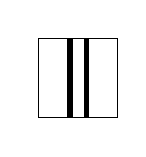
\begin{tikzpicture}
\draw[color=white, rounded corners=10, line width=8] 
(0.5, 0.0) -- (0.5, 0.5) -- (0.0, 0.5);
\draw (0, 0) -- (1, 0) -- (1, 1) -- (0, 1) -- cycle;
\draw[line width=8] 
(0.5, 0.0) -- (0.5, 1.0);
\draw[color=white, line width=4] 
(0.5, 0.0) -- (0.5, 1.0);
\end{tikzpicture}
}
\resizebox{\picwidth}{!}{
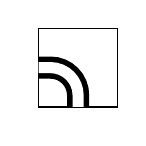
\begin{tikzpicture}
\draw (0, 0) -- (1, 0) -- (1, 1) -- (0, 1) -- cycle;
\draw[rounded corners=10, line width=8] 
(0.5, 0.0) -- (0.5, 0.5) -- (0.0, 0.5);
\draw[color=white, rounded corners=10, line width=4] 
(0.5, 0.0) -- (0.5, 0.5) -- (0.0, 0.5);
\end{tikzpicture}
}
\end{center}